% appendix/standard-normal.tex — Phi, TikZ, simplified Z-table, SciPy/Python, empirical rule; full cdf table via input
\section{The standard normal distribution}
\subsection*{A brief summary of the standard normal probability distribution}

\noindent
The \textit{cumulative distribution function} $\Phi(z)=P(Z\le z)$ equals the probability that $Z\sim N(0,1)$ falls at or below~$z$:
\[
    \Phi(z) = P(Z \le z) = \int_{-\infty}^z \phi(t) \, dt,
    \quad \text{where }\phi(z)=\frac{1}{\sqrt{2\pi}}\, e^{-z^{2}/2}.
\]

\vspace{0.45cm}
\noindent
The next figure depicts the symmetric density curve $y=\phi(z)$, the empirical rule (68--95--99.7), and shaded cumulative probability $\Phi(z)=P(Z\le z)$ left of an illustrative cutoff.

\noindent
The \textit{Simplified Standard Normal Distribution Table} (a $Z$-table) further down gives some values of $\Phi(z) = P(Z \le z)$. For example,
\[
    P(Z \le 1.7) = \Phi(1.7) = \int_{-\infty}^{1.7} \phi(z) \, dz \approx 0.9554.
\]

\begin{center}
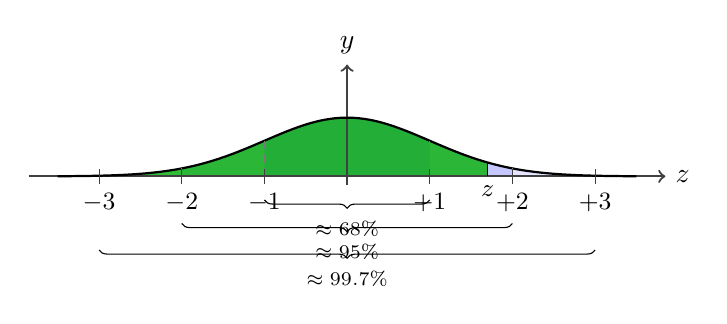
\begin{tikzpicture}[
    scale=1.05,
    yscale=1.78,
    declare function={
        normpdf(\t)=exp(-0.5*(\t)^2)/(sqrt(2*pi));
    }
]
    % Nested regions for the empirical rule (outer to inner)
    \fill[blue!10!white]
        (-3.5,0) -- plot[domain=-3.5:3.5, samples=120] (\x,{normpdf(\x)}) -- (3.5,0) -- cycle;
    \fill[blue!22!white]
        (-2,0) -- plot[domain=-2:2, samples=80] (\x,{normpdf(\x)}) -- (2,0) -- cycle;
    \fill[blue!36!white]
        (-1,0) -- plot[domain=-1:1, samples=60] (\x,{normpdf(\x)}) -- (1,0) -- cycle;
    % Cumulative probability to the illustrative boundary $z$
    \fill[green!70!black, opacity=0.78]
        (-3.5,0) -- plot[domain=-3.5:1.7, samples=72] (\x,{normpdf(\x)}) -- (1.7,0) -- cycle;
    \draw[->, thick, darkgray] (-3.85,0) -- (3.85,0) node[right, black] {$z$};
    \draw[->, thick, darkgray] (0,-0.06) -- (0,0.76) node[above, black] {$y$};
    \draw[thick, domain=-3.5:3.5, samples=120] plot (\x,{normpdf(\x)});
    \foreach \dv in {-3, -2, -1, 1, 2, 3} {
        \draw[densely dashed, darkgray!70] (\dv,0) -- (\dv,{normpdf(\dv)});
    }
    \draw (1.7,0) -- (1.7,{normpdf(1.7)});
    \foreach \tick in {-3, -2, -1} {
        \draw[darkgray] (\tick,0.05) -- (\tick,-0.05) node[below, black] {\small $\tick$};
    }
    \foreach \tick in {1, 2, 3} {
        \draw[darkgray] (\tick,0.05) -- (\tick,-0.05) node[below, black] {\small $+\tick$};
    }
    \node[below] at (1.7, 0) {\small $z$};
    % Empirical rule (68--95--99.7): braces below the axis
    \draw[decorate, decoration={brace, amplitude=3pt, mirror}]
        (-1,-0.16) -- (1,-0.16)
        node[midway, below=4pt, font=\scriptsize] {$\approx 68\%$};
    \draw[decorate, decoration={brace, amplitude=3pt, mirror}]
        (-2,-0.32) -- (2,-0.32)
        node[midway, below=4pt, font=\scriptsize] {$\approx 95\%$};
    \draw[decorate, decoration={brace, amplitude=3pt, mirror}]
        (-3,-0.50) -- (3,-0.50)
        node[midway, below=4pt, font=\scriptsize] {$\approx 99.7\%$};
\end{tikzpicture}
\end{center}

\vspace{0.6cm}

\begin{center}
{\small\textbf{Simplified Standard Normal Distribution Table}\\[0.25em]
\footnotesize\textit{(commonly known as a $Z$-table)}\\[0.65em]}
\small
\renewcommand{\arraystretch}{1.35}
\begin{tabular}{@{}c | *{10}{c}@{}}
    \toprule
    & \multicolumn{10}{c}{\textbf{first decimal place}} \\
    $z$ & .0 & .1 & .2 & .3 & .4 & .5 & .6 & .7 & .8 & .9 \\
    \midrule
    \textbf{0.} & 0.5000 & 0.5398 & 0.5793 & 0.6179 & 0.6554 & 0.6915 & 0.7257 & 0.7580 & 0.7881 & 0.8159 \\
    \textbf{1.} & 0.8413 & 0.8643 & 0.8849 & 0.9032 & 0.9192 & 0.9332 & 0.9452 & \cellcolor{purple!22}0.9554 & 0.9641 & 0.9713 \\
    \textbf{2.} & 0.9772 & 0.9821 & 0.9861 & 0.9893 & 0.9918 & 0.9938 & 0.9953 & 0.9965 & 0.9974 & 0.9981 \\
    \textbf{3.} & 0.9987 & 0.9990 & 0.9993 & 0.9995 & 0.9997 & 0.9998 & 0.9998 & 0.9999 & 0.9999 & 1.0000 \\
    \bottomrule
\end{tabular}
\end{center}

\vspace{0.35cm}
\noindent\small
\textit{Python.}
The table entries are $\Phi(z)=P(Z\le z)$ for $Z\sim N(0,1)$.
In Python~3.8+, \texttt{from statistics import NormalDist} and then \texttt{NormalDist().cdf(z)} returns these values (e.g.\ \texttt{NormalDist().cdf(1.7)} $\approx 0.9554$).
To obtain $z$ from a probability $p$ with $\Phi(z)=p$ (reading the table in reverse), use \texttt{NormalDist().inv\_cdf(p)}.

\medskip
\noindent
\textit{SciPy} (optional; \texttt{pip install scipy}). The same cdf values can be obtained with:
\begin{verbatim}
    from scipy.stats import norm

    z_score = 1.7

    # Calculate the Cumulative Distribution Function (CDF)
    probability = norm.cdf(z_score)

    # Print the result rounded to 4 decimal places
    print(f"P(Z <= {z_score}) = {probability:.4f}")
\end{verbatim}


\vspace{0.45cm}
\noindent
For many calculations the \textit{empirical rule} (68--95--99.7) is sufficient:
\begin{align*}
    P(-1 \le Z \le 1) &\approx 68\% \\
    P(-2 \le Z \le 2) &\approx 95\% \\
    P(-3 \le Z \le 3) &\approx 99.7\%
\end{align*}


\input{appendix/cumulative-z-table-full}

